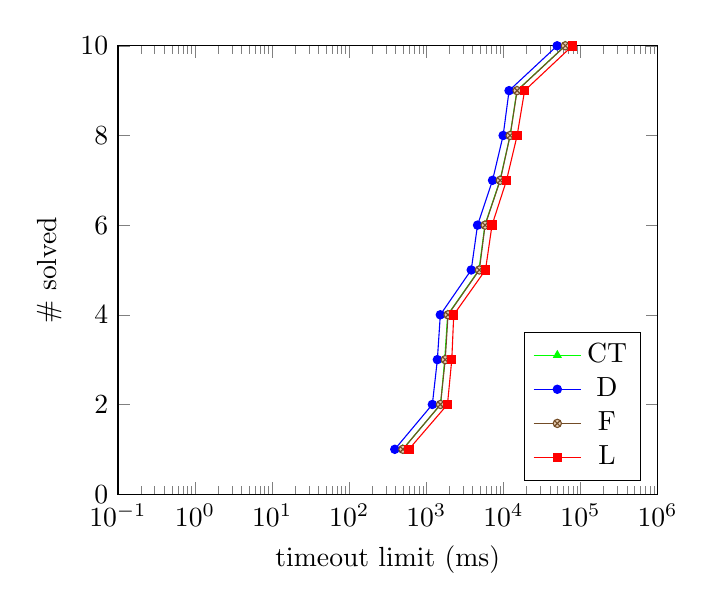
\begin{tikzpicture}[scale=1.0]
  \begin{axis}[
    xmode=log,
    ymin=0,ymax=10,
    xmin=0.1, xmax=1000000,
    every axis plot/.style={thin},
    xlabel={timeout limit (ms)},
    ylabel={\# solved},
    legend pos=south east
    % table/create on use/cumulative distribution/.style={
    %   create col/expr={\pgfmathaccuma + \thisrow{f(x)}}   
    % }
    ]
    \addplot 
    [mark=triangle*,
    mark size=1.5,
    mark options={solid},
    green] 
    coordinates {(493.707, 1)
(1534.065, 2)
(1732.300, 3)
(1892.718, 4)
(4819.172, 5)
(5753.130, 6)
(9028.954, 7)
(12217.926, 8)
(14965.073, 9)
(63087.240, 10)};

    \addplot 
    [blue,
    mark=*,
    mark size=1.5,
    mark options={solid}]
    coordinates {(390.154, 1)
(1197.210, 2)
(1390.971, 3)
(1519.242, 4)
(3823.828, 5)
(4617.781, 6)
(7228.985, 7)
(9919.531, 8)
(11845.924, 9)
(49761.700, 10)};

    \addplot [brown!60!black,
    mark options={fill=brown!40},
    mark=otimes*,
    mark size=1.5]
    coordinates {(497.095, 1)
(1524.837, 2)
(1760.207, 3)
(1913.266, 4)
(4875.522, 5)
(5784.823, 6)
(9099.779, 7)
(12223.350, 8)
(15056.924, 9)
(63609.035, 10)};

    \addplot 
    [red,
    mark size=1.5,
    mark=square*]
    coordinates {(594.196, 1)
(1881.198, 2)
(2139.673, 3)
(2268.559, 4)
(5854.235, 5)
(7115.928, 6)
(10970.686, 7)
(15071.509, 8)
(18836.865, 9)
(78418.083, 10)};
    \legend{CT,D,F,L}
  \end{axis}
\end{tikzpicture}
